\documentclass[12pt]{article}
\usepackage[shortlabels]{enumitem}
\usepackage{placeins}
\usepackage{graphicx}
\begin{document}
\title{TCES 420 - Week 8}
\author{Jake McKenzie}
\maketitle
\noindent\centerline{\textbf{Homework 7}}
\textbf{Section 1}
9.18 A certain computer provides its users with a virtual memory space of
$2^32$ bytes. The computer has $2^22$ bytes of physical memory. The virtual
memory is implemented by paging, and the page size is $4,096$ bytes.
A user process generates the virtual address $11123456$. Explain how
the system establishes the corresponding physical location. Distinguish
between software and hardware operations.\\\\
\textbf{Answer: } If we convert the virtual address from decimal to 
hex we obtain $11123456_{10}$ $=$ $0$x$00$A$9$BB$00$. We can obtain the 
page size of $2^12$ thus the first $12$ bits are for displacement within pages 
and we can deduce that the displacement within the table is $20$ bits 
because the table size is $2^20$. We obtain a $0$x$00$A$9$B for the pages 
table displacement and $0$xB$00$ for pages displacement.\\\\
9.19 Assume that we have a demand-paged memory. The page table is held in
registers. It takes 8 milliseconds to service a page fault if an empty frame
is available or if the replaced page is not modified and $20$ milliseconds if
the replaced page is modified. Memory-access time is $100$ nanoseconds.
Assume that the page to be replaced is modified $70$ percent of the
time. What is the maximum acceptable page-fault rate for an effective
access time of no more than $200$ nanoseconds?\\\\
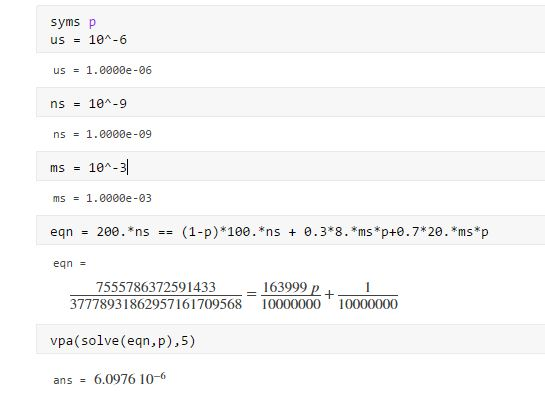
\includegraphics[scale = 1]{q19.JPG}\\
\textbf{Answer: } $p = 6.0976*10^{-6}$\\
When a page fault occurs, the process requesting the page must block
while waiting for the page to be brought from disk into physical memory.
Assume that there exists a process with five user-level threads and that
the mapping of user threads to kernel threads is one to one. If one user
thread incurs a page fault while accessing its stack, would the other
user threads belonging to the same process also be affected by the page
fault—that is, would they also have to wait for the faulting page to be
brought into memory? Explain.\\\\
\textbf{Answer: }If you have multiple threads, while one thread is blocking which is the case
in this example, the other threads in this process will be uneffected by 
the blocking.  Only on that single thread who is blocking is there an 
negative effect from the page fault.\\\\
9.22 The page table shown in Figure $9.32$ is for a system with 16-bit virtual
and physical addresses and with $4,096$-byte pages. The reference bit is
set to $1$ when the page has been referenced. Periodically, a thread zeroes
out all values of the reference bit. A dash for a page frame indicates
the page is not in memory. The page-replacement algorithm is localized
LRU, and all numbers are provided in decimal.\\\\
a) Convert the following virtual addresses (in hexadecimal) to the
equivalent physical addresses. You may provide answers in either 
hexadecimal or decimal. Also set the reference bit for the appropriate
entry in the page table.\\\\
\textbf{Answer: }\\
Virtual Address $\sim$ physical address\\
$0$xE$12$C $\sim$ $0$x$312$C\\
$0$x$3$A$9$D $\sim$ $0$xAA$9$D\\
$0$xA$9$D$9$ $\sim$ $0$x$59$D$9$\\
$0$x$7001$ $\sim$ $0$xF$001$\\
$0$xACA$1$ $\sim$ $0$x$5$CA$1$
\\\\
b) Using the above addresses as a guide, provide an example of a
logical address (in hexadecimal) that results in a page fault.\\\\
\textbf{Answer: } $0$x$4$, $0$x$8$, $0$xC and $0$xD are all page 
frames that will result in page faults
\\\\
c) From what set of page frames will the LRU page-replacement
algorithm choose in resolving a page fault?\\\\
\textbf{Answer: } I don't know how to do this and I'm completely lost.
You also won't even look at this so what even is the point.
\end{document}